%======================== 3. PROBLEM 2: FLATNESS ===============================
\isec{\faRoute}{Problem 2: Differential Flatness Trajectory Generation}

\isub{\faCalculator}{(i) Flat output and algebraic inversion}
The pursuit is planned for a unicycle model in the mission frame, which is how the chassis is commanded here
(forward speed $v$ and yaw rate $\omega$ only, eq.~(4)):
\begin{equation}
\dot x=v\cos\psi,\qquad \dot y=v\sin\psi,\qquad \dot\psi=\omega .
\end{equation}
The position $z(t)=[x(t),\,y(t)]^T$ is a flat output \cite{fliess,murray,lectures}: every state and input follows from $z$ and its derivatives
without integrating anything. The heading is the direction of the velocity, $\psi=\operatorname{atan2}(\dot y,\dot x)$,
and differentiating it gives the inputs:

\begin{keybox}{\faCalculator\ \ Flat inversion (eq.~1 of the assignment)}
\begin{equation}
v(t)=\sqrt{\dot x(t)^2+\dot y(t)^2},\qquad
\omega(t)=\dot\psi(t)=\frac{\dot x(t)\,\ddot y(t)-\dot y(t)\,\ddot x(t)}{\dot x(t)^2+\dot y(t)^2}.
\label{eq:flat}
\end{equation}
\end{keybox}
\begin{itemize}
  \item \textbf{Singularity:} at $v=0$ the heading is not defined by $z$, and $\omega$ is $0/0$. \code{flat_inversion}
        returns $\omega=0$ when $\dot x^2+\dot y^2\le10^{-6}$; the plan never stops before $t=T$, where the sample is
        held at $v=0$, $\omega=0$.
  \item \textbf{This mission:} the tag is centered before the chase, so $y(t)\equiv0$ and eq.~(\ref{eq:flat}) reduces to
        $v=\dot x$, $\omega=0$. A curved plan (for example $y(T)\neq0$) would need no code change; the offline test
        \code{test_inversion_on_circle} checks eq.~(\ref{eq:flat}) on a circle.
\end{itemize}

\isub{\faTable}{(ii) Cubic polynomial matrix solution}
Each flat component is a cubic over the horizon $T$, $z_j(t)=\alpha_0^{[j]}+\alpha_1^{[j]}t+\alpha_2^{[j]}t^2+\alpha_3^{[j]}t^3$,
$j\in\{x,y\}$. Position and velocity at both ends (Table~\ref{tab:bc}) give four linear equations:
\begin{equation}
\underbrace{\begin{bmatrix}1&0&0&0\\0&1&0&0\\1&T&T^2&T^3\\0&1&2T&3T^2\end{bmatrix}}_{\mathbf A(T)}
\begin{bmatrix}\alpha_0^{[j]}\\\alpha_1^{[j]}\\\alpha_2^{[j]}\\\alpha_3^{[j]}\end{bmatrix}
=\begin{bmatrix}z_j(0)\\\dot z_j(0)\\z_j(T)\\\dot z_j(T)\end{bmatrix},
\qquad \det\mathbf A(T)=T^4\neq0 .
\label{eq:matrix}
\end{equation}
The system has a unique solution for every $T>0$. Solving it symbolically, with $\Delta=z_j(T)-z_j(0)$:
\begin{equation}
\alpha_0=z_j(0),\quad \alpha_1=\dot z_j(0),\quad
\alpha_2=\frac{3\Delta-\big(2\dot z_j(0)+\dot z_j(T)\big)T}{T^2},\quad
\alpha_3=\frac{-2\Delta+\big(\dot z_j(0)+\dot z_j(T)\big)T}{T^3}.
\end{equation}

\begin{table}[H]
\centering\small
\rowcolors{2}{kfupmlight}{white}
\begin{tabular}{@{}lcccc@{}}
\rowcolor{kfupm}\hd{Component} & \hd{$z_j(0)$} & \hd{$\dot z_j(0)$} & \hd{$z_j(T)$} & \hd{$\dot z_j(T)$}\\
$x$ (toward the tag) & 0 & 0.06\,m/s & $d_0-0.20$ & 0\\
$y$ (left) & 0 & 0 & 0 & 0\\
\end{tabular}
\caption{Boundary conditions of the assignment, in the robot frame fixed at the start of CHASING. With all $y$ values
zero, $\bm\alpha_y=\mathbf 0$.}
\label{tab:bc}
\end{table}

The implementation solves eq.~(\ref{eq:matrix}) numerically with \code{numpy.linalg.solve}, exactly as required
(\code{rm_flatness_nav/flatness.py}, verbatim):
\begin{lstlisting}[style=py]
def solve_flat_polynomial(z0, zdot0, zf, zdotf, T):
    """Cubic coefficients [a0, a1, a2, a3] that meet position and velocity at t = 0 and t = T (eq. 2)."""
    A = np.array([
        [1.0, 0.0, 0.0, 0.0],
        [0.0, 1.0, 0.0, 0.0],
        [1.0, T, T**2, T**3],
        [0.0, 1.0, 2.0 * T, 3.0 * T**2],
    ])
    b = np.array([z0, zdot0, zf, zdotf], dtype=float)
    return np.linalg.solve(A, b)


def time_horizon(d0, v_max=V_MAX, standoff=STANDOFF, t_min=T_MIN):
    """T = max(4, 1.6 (d0 - 0.20) / v_max) (eq. 3). The 1.6 factor keeps the cubic's peak speed below v_max."""
    return max(t_min, 1.6 * (d0 - standoff) / v_max)
\end{lstlisting}
\begin{itemize}
  \item \code{FlatTrajectory(d0)} calls it once per component when CHASING starts:
        \code{alpha_x = solve_flat_polynomial(0, 0.06, d0 - 0.20, 0, T)} and
        \code{alpha_y = solve_flat_polynomial(0, 0, 0, 0, T)}.
  \item Every 50\,ms tick, \code{sample(t)} evaluates $x,\dot x,\ddot x$ (and the same for $y$) and applies
        eq.~(\ref{eq:flat}); the result is the reference $(v,\omega)$ sent to the state machine.
\end{itemize}

\begin{table}[H]
\centering\small
\rowcolors{2}{kfupmlight}{white}
\begin{tabularx}{\linewidth}{@{}>{\raggedright\arraybackslash}Xccccccc@{}}
\rowcolor{kfupm}\hd{Case} & \hd{$d_0$ (m)} & \hd{$T$ (s)} & \hd{$\alpha_0^{[x]}$} & \hd{$\alpha_1^{[x]}$} & \hd{$\alpha_2^{[x]}$} & \hd{$\alpha_3^{[x]}$} & \hd{peak $\dot x$ (m/s)}\\
% Generated by analysis/plot_flatness.py (solve_flat_polynomial).
final run, 1st chase (cut at 10.45 s) & 1.440 & 12.40 & $0$ & $0.06$ & $1.452\times10^{-2}$ & $-9.105\times10^{-4}$ & 0.1371\\
final run, chase to the stop & 1.269 & 10.69 & $0$ & $0.06$ & $1.684\times10^{-2}$ & $-1.225\times10^{-3}$ & 0.1371\\
run 011925, last chase & 1.365 & 11.65 & $0$ & $0.06$ & $1.545\times10^{-2}$ & $-1.032\times10^{-3}$ & 0.1371\\
run 012232, last chase & 1.375 & 11.75 & $0$ & $0.06$ & $1.532\times10^{-2}$ & $-1.014\times10^{-3}$ & 0.1371\\
spec lower bound & 1.500 & 13.00 & $0$ & $0.06$ & $1.385\times10^{-2}$ & $-8.284\times10^{-4}$ & 0.1371\\
spec upper bound & 1.800 & 16.00 & $0$ & $0.06$ & $1.125\times10^{-2}$ & $-5.469\times10^{-4}$ & 0.1371\\

\end{tabularx}
\caption{Coefficients $\bm\alpha_x$ from \code{solve_flat_polynomial} (units m, m/s, m/s$^2$, m/s$^3$) for the measured
$d_0$ of the floor runs and for the two ends of the assignment range. $\bm\alpha_y=\mathbf 0$ in every case. Each plan
meets $x(T)=d_0-0.20$ and $\dot x(T)=0$ to machine precision.}
\label{tab:coeff}
\end{table}

For the chase that ended the final run ($d_0=1.269$\,m, $T=10.69$\,s):
\begin{equation}
x(t)=0.06\,t+1.684\times10^{-2}\,t^2-1.225\times10^{-3}\,t^3\ \text{m},\qquad y(t)=0,
\end{equation}
with $\ddot x(0)=0.0337$\,m/s$^2$ and $\ddot x(T)=-0.0449$\,m/s$^2$: a gentle start and a gentle stop.

\isub{\faHourglassHalf}{(iii) Time horizon scaling}
\begin{equation}
T=\max\!\left(4.0,\ \frac{1.6\,(d_0-0.20)}{v_{max}}\right),\qquad v_{max}=0.16\text{\,m/s}.
\label{eq:horizon}
\end{equation}

\begin{bluebox}{\faTachometerAlt\ \ Why the factor 1.6 keeps the cruise below $v_{max}$}
\small
\begin{itemize}
  \item Let $D=d_0-0.20$ and $c=D/T$ (the mean speed). With the coefficients above, $\dot x(t)$ is a downward parabola
        with its maximum at $t^*=-\alpha_2/(3\alpha_3)$ and
        \[ \dot x_{peak}=\dot x(0)+\frac{\big(3c-2\dot x(0)\big)^2}{3\big(2c-\dot x(0)\big)} . \]
  \item \textbf{Rest to rest} ($\dot x(0)=0$): $\dot x_{peak}=1.5\,c$. A cubic that starts and ends at rest needs a peak
        50\,\% above its mean speed, so $T=1.5\,D/v_{max}$ would just touch $v_{max}$; the factor 1.6 leaves a margin:
        $\dot x_{peak}=1.5/1.6\,v_{max}=0.150$\,m/s.
  \item \textbf{With the assignment start speed} $\dot x(0)=0.06$\,m/s and $c=v_{max}/1.6=0.1$\,m/s:
        $\dot x_{peak}=0.06+0.18^2/0.42=\mathbf{0.1371}$\,\textbf{m/s} $=0.857\,v_{max}$.
  \item The peak does not depend on $d_0$ as long as the second term of eq.~(\ref{eq:horizon}) is active, that is for
        $d_0>0.60$\,m, which covers the whole 1.5 to 1.8\,m range (Table~\ref{tab:coeff}, Figure~\ref{fig:profiles}).
        Longer distances get proportionally longer horizons, not higher speeds.
  \item The 4\,s floor applies only to short distances: it keeps the start and stop accelerations bounded when $D$ is
        small.
\end{itemize}
\end{bluebox}

\begin{figure}[H]
\centering
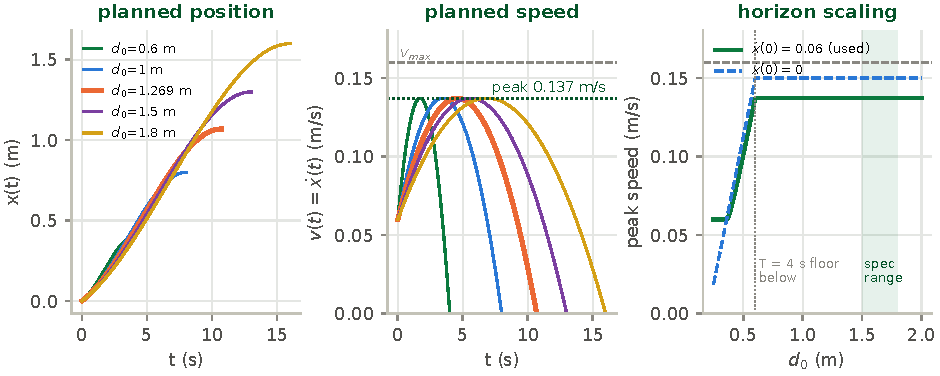
\includegraphics[width=\linewidth]{figures/p2_profiles.pdf}
\caption{Planned position and speed for several $d_0$ (bold: 1.269\,m, the final run) and the peak speed against $d_0$.
Every plan in the assignment range peaks at 0.137\,m/s, below $v_{max}$.}
\label{fig:profiles}
\end{figure}

\isub{\faChartLine}{Planned versus executed motion}
Figure~\ref{fig:planodom} compares the two plans of the final run with \code{/odom}, projected on the robot heading
at each chase start.
\begin{figure}[H]
\centering
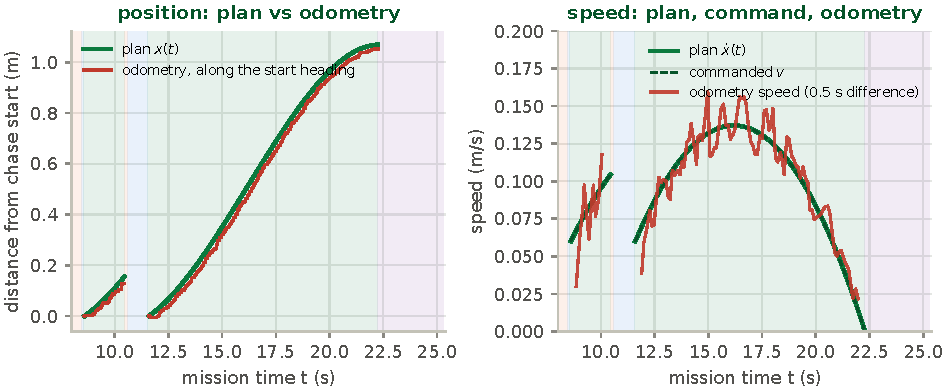
\includegraphics[width=\linewidth]{figures/p2_plan_vs_odom.pdf}
\caption{Final run: plan $x(t)$ and $\dot x(t)$ against the commanded speed and wheel odometry. The first chase
($d_0=1.440$\,m) was cut at 10.45\,s by a 2\,s detection gap; the second chase ($d_0=1.269$\,m) ran to the end of
its plan. Odometry speed is differenced over 5 \code{/odom} updates because single updates jitter over Wi-Fi.}
\label{fig:planodom}
\end{figure}
\begin{itemize}
  \item \textbf{Command = plan.} The commanded $v$ follows $\dot x_{ref}$ exactly; its maximum in the log is
        0.1371\,m/s at $t=16.05$\,s, the analytic peak.
  \item \textbf{Distance.} At the end of the plan the odometry shows 1.052\,m along the start heading and 1.060\,m in a
        straight line, against the planned 1.069\,m. Along the path, odometry trails the plan by 3.0\,cm on average
        (at most 4.8\,cm), the expected lag of a velocity-controlled chassis.
  \item \textbf{Lateral motion.} The chase began with T3 at $-9.1^\circ$ (inside the $\pm10^\circ$ tolerance). The
        bearing feedback turned the robot by $-6.7^\circ$ while driving, so it ended 13.2\,cm to the right of the
        start heading, toward the tag; the bearing at the last detection was $+0.012$\,rad.
  \item \textbf{Result.} The tape measured 20\,cm from the chassis front to the tag center after the stop.
\end{itemize}
